\begin{frame}
  \frametitle{k-Nearest Neighbors}
  \begin{adjustwidth}{-10pt}{0pt}
  \begin{minipage}{0.5\textwidth}
    \begin{block}{Objective}
      Minimum distance (\textit{Manhattan distance}) between test sample and 
      training instance(s)
    \end{block}
    \begin{block}{Algorithm hyperparameters:}
      \begin{itemize}
        \item k \textit{(1-7)}
        \item Weight of nearest neighbors: uniform or distance \textit{(distance)}
      \end{itemize}
    \end{block}
  \end{minipage}
  \hfill
  \begin{minipage}{0.5\textwidth}
    \begin{figure}
      \centering
      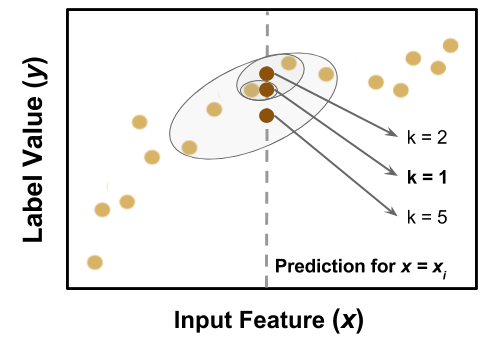
\includegraphics[height=0.5\textheight]{./figures/nn-fig.png}
    \end{figure}
  \end{minipage}
  \end{adjustwidth}
\end{frame}

\begin{frame}
  \frametitle{Decision Trees}
  \begin{adjustwidth}{-10pt}{-10pt}
  \vspace{-12pt}
  \begin{minipage}[t]{0.51\textwidth}
    \begin{block}{Objective:}
      Minimum node impurity at each split: classification uses Gini impurity,
      regression uses mean squared error
    \end{block}
  \end{minipage}%
  \hfill
  \begin{minipage}[t]{0.51\textwidth}
    \begin{block}{Algorithm hyperparameters:}
      \begin{itemize}
        \item Maximum \# of features \textit{(Feature set length, or 150)}
        \item Maximum depth \textit{(41-78)}
      \end{itemize}
    \end{block}
  \end{minipage}
    \begin{figure}
      \centering
      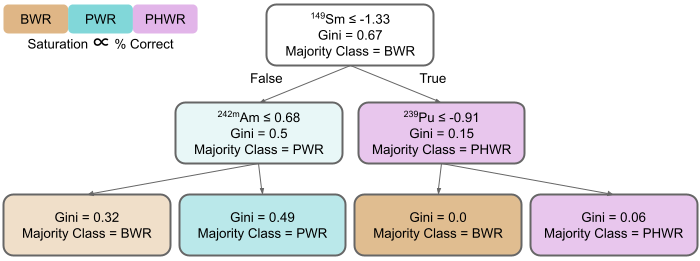
\includegraphics[width=1.05\textwidth]{./figures/dtree.png}
      Simplified example of decision tree for classification
    \end{figure}
  \end{adjustwidth}
\end{frame}

\begin{frame}
  \frametitle{Maximum Likelihood Calculations}
  \begin{block}{Objective:}
    Maximum log-likelihood value, calculated as follows:
    \[
      ln(L(M|x_{test})) = \sum_i ln(\frac{1}{\sigma_{i,train} \sqrt{2\pi}}) - 
                          \frac{(x_{i,test} - x_{i,train})^2}{2 \sigma_{i,train}^2}
    \]  
  \end{block}
  Approach based on previous work: \cite{mll_method}

\end{frame}
